% !TeX root = ../../thesis.tex

% ~5 pages 

\chapter{Introduction}
\label{chap:introduction}
From 2020 onwards all member states of the \ac{eu} are obliged to provide sensor data to the \ac{inspire} to comply with Annex II and III of the \ac{inspire} directive \citep{SDI:INSPIRE5}. For this a number of \ac{swe} standards are required to be used \citep{SDI:INSPIRE2}. The sensor web is a relatively new development and there are still many questions on how to structure it. This thesis aims to design a method to publish and link sensor metadata on the semantic web to improve the discovery, integration and aggregation of sensor data using \ac{swe} standards.


\section{Background}
In 2008 the \ac{ogc} introduced a new set of standards called Sensor Web Enablement (\ac{swe}). These standards make it possible to connect sensors to the internet and retrieve data in a uniform way. This allows users or applications to retrieve sensor data through standard protocols, regardless of the type of observations or the sensor's manufacturer \citep{SW:Botts}. Among other standards \ac{swe} includes:
\begin{itemize}
	\item \acf{om} which is a data model and encoding specification for sensor data,
	\item the \acf{sensorml} which is a model for describing sensor metadata, and
	\item the \acf{sos} which is a service for retrieving sensor data \citep{SW:OGC}.
\end{itemize}
\ac{om} has also been adopted by the \ac{iso} under \ac{iso} 19156:2011 \citep{SW:ISO}. 

Recently \ac{ogc} has defined the role which their standards could play in smart city developments \citep{SC:OGC}. Smart cities can be defined as \enquote{enhanced city systems which use data and technology to achieve integrated management and interoperability} \citep[p. 18]{SC:Moir}. Research on smart cities has shown a great potential for using sensor data in urban areas. Often this is presented in the context of the \ac{iot} \citep{IOT:Zanelli, SSW:Wang2}. The \ac{iot} can be described as \enquote{the pervasive presence around us of a variety of \textit{things} or \textit{objects} ... [which] are able to interact with each other and cooperate with their neighbors to reach common goals} \cite[p. 2787]{IOT:Atzori}. 

Parallel to the development of the sensor web, other research has focused on the semantic web, as proposed by \cite{LD:Berners-lee}. This is a response to the traditional way of using the web, where information is only available for humans to read. The semantic web is an extension of the internet which contains meaningful data that machines can understand as well. Rather than publishing documents on the web (the \textit{web of documents}), the semantic web contains linked data using the \ac{rdf}, also known as the \textit{web of data} \citep{LD:Bizer}. Data in \ac{rdf} can be queried using the \ac{sparql} at so-called \ac{sparql} endpoints. The \ac{owl} is an extension of \ac{rdf} and was designed to \enquote{represent rich and complex knowledge about things, groups of things, and relations between things} \citep{LD:OWL}. Originally, the semantic web intended to add metadata to the web \citep{LD:W3C}. However, today it is being used for linking any kind of data from one source to another in a meaningful way \citep{LD:Cambridge}. 

\cite{SSW:Sheth} propose to use semantic web technologies in the sensor web. This \ac{ssw} builds on standards by \ac{ogc} and the \ac{w3c} to \enquote{provide enhanced descriptions and meaning to sensor data} \cite[p. 78]{SSW:Sheth}. \ac{w3c} responded to this development by creating a standard ontology for sensor data on the semantic web \citep{SSW:SSN_incubatorGroup}. 


\section{Motivation}
Sensor data ties together many different fields of research. On the one hand, there is research on how to create the most efficient sensor networks that uses the least amount of energy to transfer the observed data over long distances \citep{SW:Korteweg,SW:Xiang}. This involves academic fields such as mathematics, physics and electrical engineering. On the other hand, there is research that uses sensor data to gain insights into real world phenomena. This involves academic fields such as geography, environmental studies and urbanism. To connect these scientific fields, studies have focused on the use of computer science and standardisation for transferring sensor data over the internet. 

In the future more sensor data is expected to be produced \citep{IoT:PWC}. Sensor and network technology are becoming cheaper and the required hardware increasingly smaller. This allows them to be integrated in objects that would traditionally not produce any sensor data at all, such as buildings, street lights and consumer electronics. Both experts and non-experts will be involved in this development. Organisations will produce more data and comply with \ac{swe} standards, because of the European legislation (\ac{inspire}). This involves people with expert knowledge about observations processes and online data services. Non-experts will be involved with sensor data more often in their everyday life, via smart cities and \ac{iot} developments. Non expert users and their consumer electronics are producing large amounts of sensor data as well. \cite{IOT:Barnaghi} point out that the semantic web could be of great importance for the description of sensing devices and their observations. However, \enquote{providing automated or semi-automated methods and tools to annotate, publish and access the semantic descriptions} is still described as a topic for future research \cite[p. 19]{IOT:Barnaghi}. 

The vast amount of observation data could be useful for academic research, provided researchers are able to find and combine different sources. One of the challenges of using sensor data is the difficulty of integrating data sets to perform data fusion \citep{SSW:Corcho, SSW:Ji, SSW:Wang}. Data fusion is a \enquote{data processing technique that associates, combines, aggregates, and integrates data from different sources} \cite[p. 2]{SSW:Wang2}. Even if the sources comply with the \ac{swe} standards it is challenging, because the data can be of a different granularity, both in time and space. Spatio-temporal irregularities are a fundamental property of sensor data \citep{SW:Ganesan}. 

It has been researched to what extent a catalogue service could be useful for discovering sensor data from \aclp{sos}, using the \ac{sor} \citep{SW:OGC4} and \ac{sir} \citep{SW:OGC3}. Catalogue services have already been available for the \ac{wms}, \ac{wfs} or \ac{wcs} \citep{SDI:OGC2}. However, for the sensor data sources used in this paper no register or catalogue service has been implemented. \cite{SSW:Atkinson} also argue that catalogue services have a number of major disadvantages. It places a very high burden on the client to not only know where to find the catalogue service, but also to have knowledge on all kinds of other aspects (e.g. its organisation, access protocol, response format and response content) \cite[p. 128]{SSW:Atkinson}. 

\citeauthor{SSW:Atkinson} suggest that linked data is a much better solution for discovering sensor data. When publishing sensor metadata on the semantic web, it is easier to find related resources. Furthermore, the added meaning required to publish it on the semantic web, can be helpful in harmonising sensor data from different sources. This allows multiple sources to be integrated on-the-fly, based on their semantic descriptions. Having automated processes to perform these tasks, could be of great use for research as performed by \cite{UC:vanderHoeven}, \cite{UC:Hotterdam} and \cite{UC:Theunisse}. They are examples of studies which try to understand phenomena in the built environment using sensor data. Currently data collection and processing takes up a large part of the research, while with the implementation of \ac{swe} standards and the use of the semantic web this can be significantly reduced.  

%At the moment, finding sensor data which can be retrieved using open standards is challenging and the implementation of the sensor web is still at an early stage. A number of organisations still use custom \acp{api} to retrieve data from sensors connected to the internet. The problem with these custom \ac{api}s is that it is very hard to create web applications that automatically retrieve data from them, because they have not implemented standards regarding the content of their service, the metadata models behind it or the kind of requests that can be made. It forces an application to have knowledge built in on the specifics of the individual \ac{api}s that are being used.  

The question could be raised to what extent the semantic web is a better solution for publishing observation data and should replace the current geoweb solutions like \ac{sos}. Apart from the issues mentioned above, the geoweb has some very good qualities. It offers very structured approaches through which large amounts of (sensor) data can be retrieved using well defined services. These standardised services have been accepted by important organisations like \ac{ogc} and \ac{iso}. They are often based on years of discussion by professional communities. Furthermore, the response of a \ac{sos} also contains a certain amount of semantics about sensor data. So-called x-links can be placed inside the \ac{xml} with \ac{uri}s that point to semantic definitions of objects. Therefore, the geoweb solutions like \ac{sos} should not be disregarded.

Still, the semantic web could be beneficial in combination with the geoweb. Since data on the web has a distributed nature it can be questioned whether centralised catalogue services are feasible to create. It places a burden on the owner of the \ac{sos} to register at a catalogue service. Also, there could be multiple of these services on the web creating issues regarding the discovery of relevant catalogues. The semantic web could solve this issue by getting rid of the information silos and storing data directly on the web instead. This allows the interlinking and reuse of data on the web, which makes it easier to find related data. Having semantic descriptions of observation metadata makes it easier to harmonise and combine different sources. For automatic processes to find, retrieve and aggregate observations it is useful that the semantic web is machine understandable. 

However, for sensor data to be discovered on the semantic web there have to be inward links from other sources linking towards the sensor (meta)data. Current research on the \ac{ssw} has focused on publishing sensor data on the semantic web with links that point outwards \citep{SSW:Janowicz, SSW:Pschorr, SSW:Atkinson}. Although this gives meaning to the data and can be used to harmonize \ac{sos} content, it has a very limited effect on the discovery of sensor data by others. Therefore, to discover, integrate and aggregate data from multiple sources, both inward and outward links are needed.  

As sensor data is becoming more important the gap between the logical data queries of users and the technical requests defined by sensor web protocols should be bridged. A logical sensor data query contains at least a geographical area, a type of observation and a time range. For example: \textit{What are the average particulate matter levels per month in neighbourhoods of Delft over the last five years?} To translate this to a technical request specific knowledge is required about things like \acp{uri}, encodings, data models, service models and data formats. This thesis uses the semantic web to enable automated processes to perform this translation to \ac{sos} requests. Figure \ref{fig:logical} shows the web application that has been created in this thesis as an interface for automatically finding and retrieving data from \aclp{sos}, using the semantic web. 


\begin{figure}
	\centering
	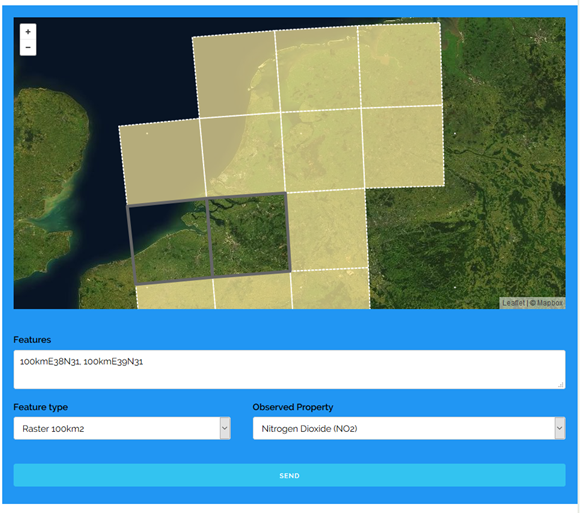
\includegraphics[width=0.8\linewidth]{figs/interface1.PNG}
	\caption{Web application created in this thesis, which uses the semantic to find and retrieve sensor data from \aclp*{sos} based on logical input.}
	\label{fig:logical}
\end{figure}


\section{Thesis objectives}
There is still a lack of knowledge on how to exploit the full potential of the sensor web using the semantic web. Converting \ac{sos} metadata to linked data could greatly enhance the discovery, integration and aggregation of sensor data. However, there is no method yet to establish this linked metadata for sensors, while the standardised nature of a \ac{sos} should enable it to be created in an automated process. This thesis presents a design for such an automated process and explores the advantages and disadvantages of publishing sensor metadata on the semantic web with a proof-of-concept implementation. 

When using observation data for studying phenomena in a border region, it is important to have data about both sides. Moreover, borders are a social construct and do not influence natural phenomena such as air quality. Therefore, two \aclp{sos} have been used in this thesis, containing complementary air quality data of the Netherlands and Belgium (Figure \ref{fig:combined}). The first source is the \ac{sos} by the \ac{rivm}. It has recently been launched and is one of the first \ac{swe} services to become available in the Netherlands. The second \ac{sos} is maintained by the \acf{ircel}. \ac{ircel} has been making air quality sensor data available using a \ac{sos} for a number of years already. Both of these services have been used to answer the research questions.


% Research question 
\section{Research questions}
\label{RQ}
This thesis aims to design a conceptual system architecture that uses the semantic web to improve sensor data discovery as well as the integration and aggregation of sensor data from multiple sources. The following question will be answered in this research:    

\begin{quote}
	\textit{To what extent can the semantic web improve the discovery, integration and aggregation of distributed sensor data?}
\end{quote}

To answer the main question, four subquestions have been specified:
\begin{itemize}
	\item To what extent can sensor metadata be automatically retrieved from any \acl{sos}?
	\item To what extent can sensor metadata from a \acl{sos} be automatically converted to linked data and published on the semantic web?
	\item  What is an effective balance between the semantic web and the geoweb in the chain of discovering, retrieving and processing sensor data?
	\item To what extent can already existing standards for retrieving data be (re)used for a service that supplies integrated and aggregated sensor data?
\end{itemize}

\begin{figure}
	\centering
	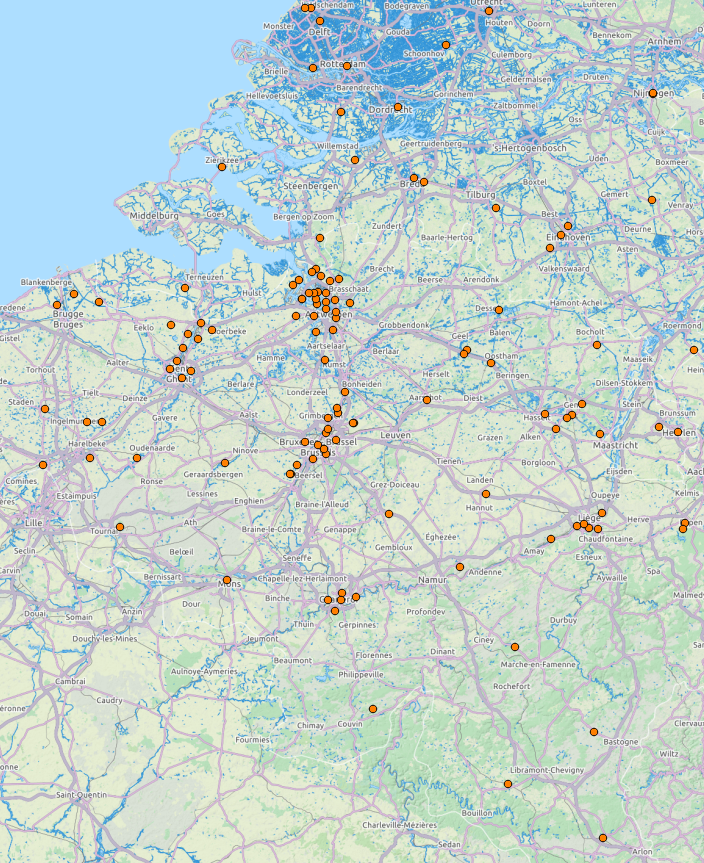
\includegraphics[width=\linewidth]{figs/combined.png}
	\caption{The combined air quality sensor network of the \aclp*{sos} of the \acf*{ircel} and the \acf*{rivm} in Belgium and the South of the Netherlands.}
	\label{fig:combined}
\end{figure}




